\documentclass[letterpaper,11pt]{article}
\usepackage[spanish]{babel}
\usepackage[utf8]{inputenc}
\usepackage{graphicx}
\usepackage{amsfonts,amsmath,amssymb,float, amsthm,mathrsfs}  
\usepackage[right=4.5cm,left=2cm,top=3cm,bottom=3cm,headsep= 0.7cm,footskip=0.5cm]{geometry}
\usepackage{enumerate}
\usepackage{wrapfig} 
\usepackage[rflt]{floatflt} 
\usepackage{framed}
%\usepackage[most]{tcolorbox}
\usepackage[dvipsnames]{xcolor}
\colorlet{shadecolor}{green!20}
\setlength\FrameSep{0.5ex}
\usepackage{thmtools}
\usepackage{esint}
\usepackage{cancel}
\usepackage{listings} 
\usepackage{pstricks, caption}
\usepackage[colorlinks]{hyperref}
\usepackage{csquotes}
\usepackage{fullpage}
\usepackage{enumitem}
\usepackage{etoolbox}
\usepackage{tikz}
\usepackage{tikz-3dplot}
\tdplotsetmaincoords{80}{70}
\usetikzlibrary{decorations.markings}
\usetikzlibrary{arrows,babel}
\usepackage[font=small]{caption}
\usepackage{scalerel} %\scaleto{text}{size}
\usepackage{subfigure}
\usepackage{fancyhdr}
\usepackage{comment}
\usepackage{marginnote}
\usepackage{tensor}
\usepackage{cleveref}
\newcommand{\dbar}{\mathchar'26\mkern-12mu d}
\renewcommand*{\marginnotevadjust}{-0.1cm}
\renewcommand*{\marginfont}{\footnotesize}
\setlength{\headheight}{15pt}
\addtolength{\topmargin}{-14.49998pt}
\setlength{\headsep}{15pt}
\setlength{\footskip}{14.49998pt}
\decimalpoint
\newcommand{\grad}{^\circ}
\newlength{\drop}
\DeclareMathOperator{\sign}{sgn}
\DeclareMathOperator{\Log}{Log}
\providecommand{\norm}[1]{\lVert#1\rVert}

\let\cancelorigcolor\CancelColor% Just for conveniency...

\newcommand{\CancelTo}[3][]{%
  \ifblank{#1}{}{%
    \renewcommand{\CancelColor}{#1}%
  }
  \cancelto{#2}{#3}% 
}


\begin{document}

\pagestyle{plain}

\begin{flushleft}\vspace{-2cm}
Departamento de Física \\
Facultad de Cs. Físicas y Matemáticas\\
Universidad de Concepción
\end{flushleft}

\begin{flushright}\vspace{-1.5cm}
\textbf{Tópicos en Relatividad General} 
\end{flushright}



\rule{\linewidth}{0.1mm}

\begin{center}
\textbf{\LARGE Semana 4}
\end{center}

\begin{flushleft}
\textbf{Nombre:} Alejandro Saavedra San Martín. \\
\textbf{Profesor:} Guillermo Rubilar Alegría.
\end{flushleft}

\section*{Órbitas ligadas no-circulares}

Si $h > 2 \sqrt{3}$, $\tilde{V}(r_B) < k^2 < \tilde{V}(r_A)$ y $k < 1$, existen órbitas ligadas, cuyas coordenadas radiales varían entre $r_{\text{mín}}$ y $r_{\text{máx}}$, con $\tilde{V}(r_{\text{mín}}) = \tilde{V}(r_{\text{máx}}) = k^2$, ver figura \ref{fig:Potential}. 

\begin{figure}[H] 
    \centering
    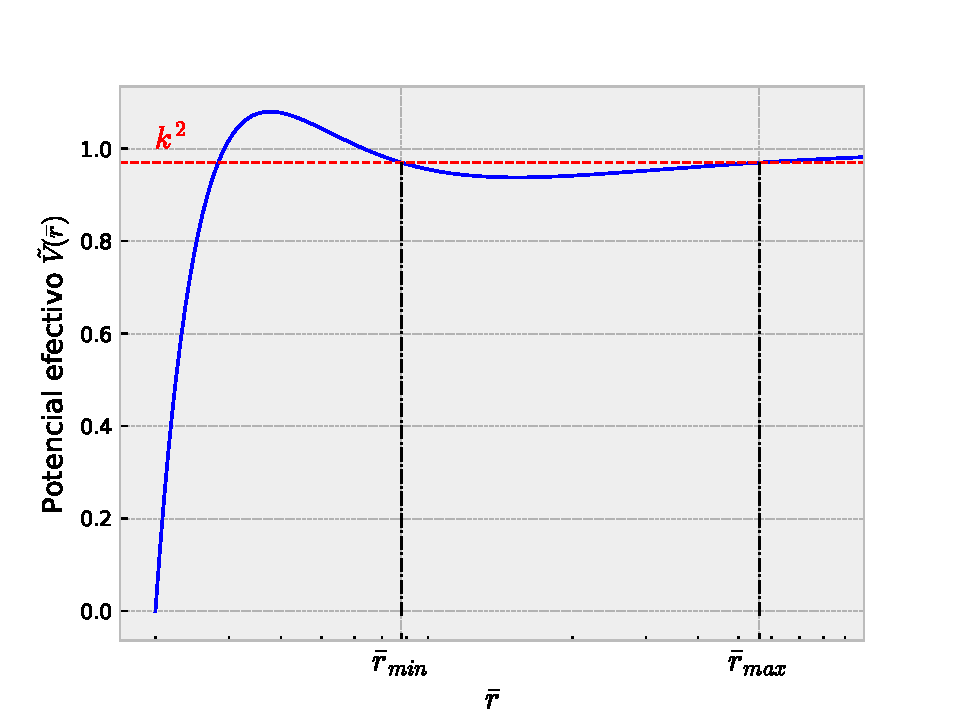
\includegraphics[scale = 0.7]{Potencial_Efectivo_orbita-ligada}
    \caption{Potencial efectivo para órbitas ligadas.}
    \label{fig:Potential}
\end{figure}

Para analizar la forma de la trayectoria consideremos que la coordenada radial en términos de la angular, $r = r(\varphi)$. Por regla de la cadena,
\begin{equation}
\dot{r} = \frac{dr}{d\varphi} \frac{d\varphi}{d\tau} = r' \dot{\varphi},
\end{equation}

donde $r' := dr/d\varphi$. Como $hmc = r^2 \sin\theta \dot{\varphi} = r^2 \dot{\varphi}$, 
\begin{equation}
hmc = r^2 \frac{\dot{r}}{r'}.
\end{equation}

Así,
\begin{equation} \label{eq:r-derivative}
\dot{r} = \frac{hmc}{r^2} r'.
\end{equation}

Derivando con respecto a $\tau$ la ecuación \eqref{eq:r-derivative}, obtenemos
\begin{align}
\ddot{r} &= - \frac{2 hmc}{r^3} r' \dot{r} + \frac{hmc}{r^2} r'' \dot{\varphi} \nonumber \\
&= - \frac{2 hmc}{r^3} r' \left( \frac{hmc}{r^2} r' \right) + \frac{hmc}{r^2} r'' \left( \frac{hmc}{r^2} \right) \nonumber \\
&= - 2 h^2m^2c^2 \frac{r'\,^2}{r^5} + h^2m^2c^2 \frac{r''}{r^4}\nonumber  \\
&= \frac{h^2m^2c^2}{r^2} \left( - \frac{2}{r} r'\,^2 + r'' \right). \label{eq:r-second-derivative}
\end{align}

Al igual que en el caso newtoniano, definimos la variable auxiliar
\begin{equation} \label{eq:def-u}
u := \frac{1}{r}.
\end{equation}

Derivando con respecto a $\varphi$:
\begin{equation}
u' = - \frac{r'}{r^2} = - u^2 r'.
\end{equation}

Así,
\begin{equation} \label{eq:derivative-u}
r' = - \frac{1}{u^2} u'.
\end{equation}

Luego, la segunda derivada es
\begin{align}
u'' &= \frac{d}{d\varphi} (-u^2 r') \nonumber \\
&= -2 u u' r' - u^2 r'' \nonumber \\
&=  -2 u u' \left(- \frac{u'}{u^2} \right) - u^2 r'' \nonumber \\
&= 2 \frac{u'\,^2}{u} - u^2 r''.
\end{align}

Despejando $r''$:
\begin{equation} \label{eq:2nd-derivative-u}
r'' = \frac{2}{u^3} u'\,^2 - \frac{1}{u^2} u''.
\end{equation}

En el documento de la semana 3 encontramos que la dinámica de la coordenada $r$ está determinada por la ecuación
\begin{equation}
\dot{r}^2 = k^2c^2 - c^2 \left(1 - \frac{2m}{r}\right)\left(1 + \frac{h^2m^2}{r^2}\right).
\end{equation}

Usando \eqref{eq:r-derivative}, \eqref{eq:def-u} y \eqref{eq:derivative-u}, encontramos que 
\begin{align}
\frac{h^2m^2\cancel{c^2}}{r^4} r'\,^2 &= k^2\cancel{c^2} - \cancel{c^2} \left(1 - \frac{2m}{r} \right)\left(1 + \frac{h^2m^2}{r^2}\right) \\
h^2m^2u^4 \left(-\frac{1}{u^2} u' \right) &= k^2 - (1-2mu)(1+h^2m^2u^2). 
\end{align} 

Entonces,
\colorlet{shadecolor}{green!20}
\begin{shaded}
\begin{equation} \label{eq:motion-u'}
h^2m^2u'\,^2 - k^2 + (1-2mu)(1+h^2m^2u^2) = 0.
\end{equation}
\end{shaded}

Derivando con respecto a $\varphi$ la ecuación \eqref{eq:motion-u'}:
\begin{align}
2h^2m^2u' u'' - 2mu' (1+h^2m^2u^2) + (1-2mu)(2h^2m^2uu') &= 0 \\
2h^2m^2u' u'' - 2mu' - 2h^2m^3u^2u' + 2h^2m^2uu' - 4h^2m^3u^2u' &= 0 \\
h^2m^2 u' u'' - m u' - 3h^2m^3 u^2 u' + h^2m^2 u u' &= 0 \\
h^2m^2 u' u'' + h^2m^2 u u' &=  m u' + 3h^2m^3 u^2 u' \\
 u' u'' +  u u' &=  \frac{1}{h^2 m} u' + 3m u^2 u'.
\end{align}

Ahora, si no consideramos órbitas circulares, $r$ no constante, con $u' \neq 0$, obtenemos que
\begin{shaded}
\begin{equation} \label{eq:motion-u''}
u'' + u = \frac{1}{h^2m} + 3mu^2.
\end{equation}
\end{shaded}

Si definimos la variable adimensional
\begin{equation}
w := h^2m u.
\end{equation}

La ecuación \eqref{eq:motion-u''} puede escribirse como
\begin{align}
\frac{1}{h^2m} w'' + \frac{1}{h^2m} w &= \frac{1}{h^2m} + \frac{3m}{m^2h^4} w^2 \\
w'' + w &= 1 + \frac{3}{h^2} w^2.
\end{align}

Finalmente, si $\epsilon:= 3/h^2$, entonces 
\begin{shaded}
\begin{equation} \label{eq:motion-u''}
w'' + w = 1 + \epsilon w^2.
\end{equation}
\end{shaded}
\end{document}
